\documentclass[11pt]{article}
\usepackage[margin=1in]{geometry}
\usepackage{amsmath,amssymb,amsthm}
\usepackage{booktabs}
\usepackage{hyperref}
\usepackage{tikz}

\newtheorem{theorem}{Theorem}
\newtheorem{lemma}[theorem]{Lemma}
\newtheorem{definition}[theorem]{Definition}
\newtheorem{remark}[theorem]{Remark}

\title{Threshold Output Preservation under Bounded Score Perturbations}
\author{Research Architecture Runtime \\ \texttt{feature/lean-gated-operator-papers}}
\date{2026-07-25}

\begin{document}
\maketitle

\begin{abstract}
We study the scalar thresholding operator
\(A_T(x)=\mathbf{1}\{x\ge T\}\) under additive score perturbations
with \(\lvert x'-x\rvert\le\varepsilon\).
Because equality passes, preservation is asymmetric:
\(x\ge T+\varepsilon\) guarantees output \(1\), while
\(x<T-\varepsilon\) (strict) guarantees output \(0\).
On the half-open unstable band \([T-\varepsilon,T+\varepsilon)\) the
decision need not be invariant; we exhibit sharp one-dimensional
counterexamples.
Publication is gated on Lean \texttt{LEAN\_FULL} for
\texttt{Research.Operators.Threshold.Preservation.threshold\_preservation}
(Mathlib $\mathbb{R}$; \texttt{REAL\_MATHLIB}).
\end{abstract}

\section{Introduction}
Thresholding is a canonical selection primitive in adaptive data analysis
and differential privacy (AboveThreshold / Sparse Vector).
Before noisy sequential mechanisms, the deterministic scalar rule already
exhibits a clear decision boundary \(x=T\) and a margin-controlled
robustness statement.
This note records that statement as an operator-specific theorem exercised
end-to-end through Discovery and Verification in this repository.

\section{Problem formulation}
Fix a threshold \(T\in\mathbb{R}\) and a score \(x\in\mathbb{R}\).
Define
\[
A_T(x)=\mathbf{1}\{x\ge T\}.
\]
\paragraph{Equality convention.}
\(A_T(x)=1\) if and only if \(x\ge T\) (equality counts as a pass).
\paragraph{Perturbation model.}
Admissible neighbors satisfy \(\lvert x'-x\rvert\le\varepsilon\) for
\(\varepsilon\ge 0\).
Non-finite scores or thresholds are rejected by the implementation.

\section{Notation and definitions}
\begin{definition}[Signed margin and distance]
\(m(x)=x-T\) and \(d(x)=\lvert x-T\rvert\).
\end{definition}
\begin{definition}[Preservation predicates]
Pass is preserved if every admissible \(x'\) satisfies \(A_T(x')=1\).
Fail is preserved if every admissible \(x'\) satisfies \(A_T(x')=0\).
\end{definition}

\section{Mathematical assumptions}
\begin{enumerate}
\item \(x,T\in\mathbb{R}\) are finite.
\item \(\varepsilon\ge 0\) and \(\lvert x'-x\rvert\le\varepsilon\).
\item Equality convention \(x\ge T\) passes.
\end{enumerate}
We do not treat data-dependent maps \(x(D)\) beyond the abstract score,
nor Sparse Vector privacy accounting in this note.

\section{Main theorem}
\begin{theorem}[Threshold output preservation]\label{thm:main}
Under the assumptions above:
\begin{enumerate}
\item If \(x\ge T+\varepsilon\), then \(A_T(x')=1\).
\item If \(x<T-\varepsilon\), then \(A_T(x')=0\).
\item If \(x\in[T-\varepsilon,T+\varepsilon)\), the output need not be invariant.
\end{enumerate}
\end{theorem}

\begin{theorem}[Sharpness with equality asymmetry]\label{thm:sharp}
\begin{enumerate}
\item If \(x\in[T,T+\varepsilon)\), then \(x'=x-\varepsilon\) is admissible and
\(A_T(x')=0\).
\item If \(x\in[T-\varepsilon,T)\), then \(x'=x+\varepsilon\) is admissible and
\(A_T(x')=1\).
\item At \(x=T+\varepsilon\), every admissible \(x'\) satisfies \(A_T(x')=1\)
(pass-side condition is non-strict).
\item At \(x=T-\varepsilon\), fail is \emph{not} preserved (since \(x'=T\) passes).
\end{enumerate}
\end{theorem}

\section{Supporting lemmas}
\begin{lemma}[Interval image]\label{lem:interval}
The set of admissible \(x'\) is the closed interval \([x-\varepsilon,x+\varepsilon]\).
\end{lemma}
\begin{proof}
Immediate from \(\lvert x'-x\rvert\le\varepsilon\).
\end{proof}

\section{Proofs}
\begin{proof}[Proof of Theorem~\ref{thm:main}]
If \(x\ge T+\varepsilon\), then \(x-\varepsilon\ge T\), so every \(x'\ge T\) and
\(A_T(x')=1\).
If \(x<T-\varepsilon\), then \(x+\varepsilon<T\), so every \(x'<T\) and
\(A_T(x')=0\).
If \(x\in[T-\varepsilon,T+\varepsilon)\), the interval
\([x-\varepsilon,x+\varepsilon]\) intersects both \(\{y:y<T\}\) and
\(\{y:y\ge T\}\) (or, at the left endpoint, reaches \(T\)), so both outputs
are attainable except on the empty \(\varepsilon=0\) band.
\end{proof}

\begin{proof}[Proof of Theorem~\ref{thm:sharp}]
For \(x\in[T,T+\varepsilon)\), \(x-\varepsilon<T\), hence \(A_T(x-\varepsilon)=0\).
For \(x\in[T-\varepsilon,T)\), \(x+\varepsilon\ge T\), hence \(A_T(x+\varepsilon)=1\).
At \(x=T+\varepsilon\), \(x-\varepsilon=T\) still passes.
At \(x=T-\varepsilon\), \(x+\varepsilon=T\) passes, so fail is not invariant.
\end{proof}

\section{Discussion}
\subsection{Intuition}
The threshold is a hard cut. A buffer of size \(\varepsilon\) on the correct side
of \(T\) absorbs worst-case movement toward the cut.
Because the cut includes equality, the pass buffer is closed on the left
(\(x\ge T+\varepsilon\)) while the fail buffer is open (\(x<T-\varepsilon\)).

\subsection{Geometric explanation}
\begin{figure}[h]
\centering
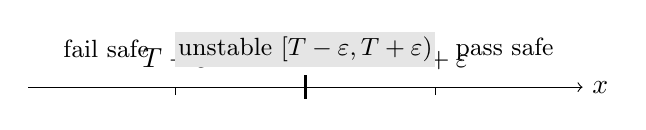
\begin{tikzpicture}[xscale=1.1]
\draw[->] (-3.2,0) -- (3.2,0) node[right] {\(x\)};
\draw[thick] (0,-0.15) -- (0,0.15) node[above] {\(T\)};
\draw[dashed] (-1.5,-0.1) -- (-1.5,0.1) node[above] {\(T-\varepsilon\)};
\draw[dashed] (1.5,-0.1) -- (1.5,0.1) node[above] {\(T+\varepsilon\)};
\fill[gray!20] (-1.5,0.25) rectangle (1.5,0.7);
\node[font=\small] at (0,0.48) {unstable \([T-\varepsilon,T+\varepsilon)\)};
\node[font=\small] at (-2.3,0.48) {fail safe};
\node[font=\small] at (2.3,0.48) {pass safe};
\end{tikzpicture}
\caption{Asymmetric preservation regions for \(A_T(x)=\mathbf{1}\{x\ge T\}\).}
\label{fig:regions}
\end{figure}

\subsection{Why it matters}
A measured margin \(m=x-T\) is an operational certificate for selection
stability under bounded score noise---the scalar core of AboveThreshold.

\subsection{Where assumptions are used}
Finiteness excludes \(\mathrm{NaN}/\pm\infty\); the equality convention forces
the half-open unstable band; \(\varepsilon\ge 0\) covers the trivial invariant case
\(\varepsilon=0\).

\subsection{Examples}
Take \(T=0\), \(\varepsilon=1\). Then \(x=2\) and \(x=1\) are pass-safe;
\(x=0.5\), \(x=0\), \(x=-0.5\), \(x=-1\) are unstable; \(x=-2\) is fail-safe.

\subsection{Counterexamples and boundary cases}
At \(x=T+\varepsilon\) pass cannot be broken.
At \(x=T-\varepsilon\) the adversary \(x'=T\) flips a fail to a pass.

\section{Interpretation}
Compare \(\lvert m\rvert\) to \(\varepsilon\) with the stated asymmetry before
trusting a reported pass/fail bit under score uncertainty.

\section{Utility implications}
Abstention bands use the same asymmetry as preservation: release \(1\) only when
\(x\ge T+\tau\), release \(0\) only when \(x<T-\tau\), else \(\bot\).
(The naive closed fail rule \(x\le T-\tau\) is \emph{not} robust at \(x=T-\tau\) when
\(\varepsilon=\tau\).) Set-valued selectors \(\{0\}\), \(\{1\}\), \(\{0,1\}\) match
the preservation predicates.

\section{Noisy and sequential extensions}
Noisy mechanisms (query noise, threshold noise, both), abstention, and
first-crossing \(\widetilde\tau\) are implemented as a portfolio.
A companion note verifies bounded almost-sure noise pathwise.
Full Sparse Vector privacy is \textbf{not} claimed here.

\section{Limitations}
\begin{itemize}
\item Lean formalization is Mathlib $\mathbb{R}$ (\texttt{REAL\_MATHLIB}).
\item Scalar finite scores only.
\item Sparse Vector / adaptive positive-release accounting not verified.
\end{itemize}

\section{Open questions}
Adaptive query order, limited positive releases, likelihood-ratio stability
parameters, and full Sparse Vector theorems.

\section{Connections to existing framework}
Discovery IR \(\to\) sealed CRP \(\to\) System~B \(\to\) System~3 Lean
(\texttt{Research.Operators.Threshold.Preservation}).
Certificate:
\texttt{lean/certificates/thresholding/threshold-output-preservation/}.

\section{Verifier summary}
Publication requires \texttt{LEAN\_FULL} (sorry/admit \(=0\), \texttt{build\_ok}).
Prior computational-only paper archived under \texttt{\_archive/v0-computational/}.

\section{Appendix}
Canonical statement (repository string):
\begin{quote}\small
Let \(x,x'\in\mathbb{R}\) and \(\varepsilon\ge 0\) with \(\lvert x'-x\rvert\le\varepsilon\).
For \(A_T(x)=\mathbf{1}\{x\ge T\}\) with fixed \(T\in\mathbb{R}\):
(1) if \(x\ge T+\varepsilon\) then \(A_T(x')=1\);
(2) if \(x<T-\varepsilon\) then \(A_T(x')=0\);
(3) if \(x\in[T-\varepsilon,T+\varepsilon)\) the output need not be invariant.
\end{quote}

\section*{References}
\begin{thebibliography}{9}
\bibitem{dwork2014}
Dwork, C., and Roth, A.
\emph{The Algorithmic Foundations of Differential Privacy}.
Foundations and Trends in Theoretical Computer Science, 2014.
(AboveThreshold / Sparse Vector as noisy thresholding primitives.)
\bibitem{repo}
Repository implementation:
\texttt{implementation/src/operators/thresholding/}.
\end{thebibliography}

\end{document}
